% Dies ist Teil der Vorlesung Physik auf dem Computer, SS 2012,
% Axel Arnold, Universitaet Stuttgart.
% 
% Dieses Werk ist unter einer Creative Commons-Lizenz vom Typ
% Namensnennung-Weitergabe unter gleichen Bedingungen 3.0 Deutschland
% zugänglich. Um eine Kopie dieser Lizenz einzusehen, konsultieren Sie
% http://creativecommons.org/licenses/by-sa/3.0/de/ oder wenden Sie sich
% schriftlich an Creative Commons, 444 Castro Street, Suite 900, Mountain
% View, California, 94041, USA.

\chapter{Nichtlineare Gleichungssysteme}
\index{Nullstellensuche}
\index{Fixpunktsuche}

Im zweiten Kapitel hatten wir uns mit der Lösung linearer
Gleichungssysteme beschäftigt, die ja eine wesentliche Grundlage der
numerischen Mathematik darstellen. Allerdings tauchen in der Praxis,
besonders in der Physik, leicht auch nichtlineare Gleichungssysteme
auf. In diesem Fall kann man meist keine allgemeine Aussage über
Existenz und Anzahl der Lösungen machen, und kann auch keine exakten
Verfahren zur Lösung angeben.

Nichtlineare Gleichungssysteme werden typischerweise in zwei Formen
betrachtet. Sei eine Funktion $f:M\in\RR^n\to\RR^n$ gegeben. Dann suchen
wir die \emph{Nullstellen}
\begin{equation}
  \label{eq:nullstellen}
  x, \quad\text{so dass}\; f(x) = 0,
\end{equation}
also die Lösungen zur Gleichung $f(x) = 0$. Man beachte, dass anders
als im Fall der linearen Gleichungssysteme gefordert wird, dass der
Bildraum wie auch der Ursprungsraum $M$ zu einem Vektorraum derselben
Dimension $n$ gehören. Ohne diese Voraussetzung ist eine eindeutige
Lösung im allgemeinen unmöglich. Anders als im Falle der linearen
Gleichungssysteme ist es hier auch nicht ohne weiteres möglich, den
Lösungsraum anzugeben, falls die Lösung nicht eindeutig
ist. Tatsächlich kann der Lösungsraum ja einen beliebig komplexe
Mannigfaltigkeit innerhalb $M$ darstellen, die dann gar nicht
geschlossen parametrisiert werden kann. Das macht die numerische
Bestimmung dieser Lösungsmannigfaltigkeit sehr schwierig.

Alternativ können wir für eine Funktion $g:M\in\RR^n\to\RR^n$ die
\emph{Fixpunkte} suchen. Diese sind
\begin{equation}
  \label{eq:fixpunkt}
  x, \quad\text{so dass}\; g(x) = x,
\end{equation}
also die Lösungen der Gleichung $g(x) = x$. Eine Fixpunktgleichung
lässt sich natürlich stets auch als Nullstellenproblem mit $f(x) =
g(x) - x$ formulieren; anders herum geht dies im allgemeinen nicht.

Die beiden Formulierungen unterscheiden sich allerdings im natürlichen
Lösungsansatz. Die Nullstellengleichung \eqref{eq:nullstellen} ähnelt
dem linearen Gleichungssystem \eqref{eq:lgs}. Das
\emph{Newtonverfahren} beruht auf einer lokalen Linearisierung und dem
Lösen dieses linearen Gleichungssystems. Die Fixpunktgleichung
hingegen legt nahe, den Fixpunkt durch \emph{sukzessive Substitution}
zu suchen: $x_0\to g(x_0)\to g(g(x_0))\to\ldots$.

\section{Sukzessive Substitution}
\index{sukzessive Substitution}
\index{Fixpunktsuche}

Eine Abbildung $g:M\to M$ mit $M\subset\RR^n$ heißt Lipschitz-stetig
(L-stetig), falls es ein $L\in\RR$ gibt, so dass
\begin{equation}
  \norm{g(x) - g(y)} \le L \norm{x - y}\quad\forall x,y\in M.
\end{equation}
Alle auf $M$ differenzierbaren Funktionen mit beschränkter Ableitung
sind L-stetig, wenn ihre Ableitung beschränkt ist. Die
Lipschitzkonstante ergibt sich aus dem Mittelwertsatz zu $L=\max_{x\in
  M}\norm{g'(x)}$.  Es gibt allerdings noch mehr L-stetige Funktionen,
zum Beispiel die in 0 nicht differenzierbare Betragsfunktion, die auf
ganz $\RR$ L-stetig mit $L = 1$ ist. Auf der anderen Seite ist
offenbar jede L-stetige Funktion auch stetig, d.h., die L-stetigen
Funktionen sind eine eigene Klasse zwischen den stetigen und
differenzierbaren Funktionen.

\index{Banachscher Fixpunktsatz} Hat eine Funktion $g:M\to M$ eine
Lipschitz-Konstante $L<1$, so heißt $g$ \emph{kontrahierend}, weil
zwei verschiedene Punkte durch die Abbildung stets näher aneinander
geschoben werden. Wir betrachten nun einen beliebigen Startpunkt
$x_0\in M$ und definieren damit die Folge der \emph{sukzessive Substitution}:
\begin{equation}
  x_{n} := g(x_{n-1}) \quad\text{für}\; n\ge 1.
\end{equation}
Dann gilt für alle $n,m\in\NN$ der \emph{Banachsche Fixpunktsatz}
\begin{align}
  \label{eq:banach}
  \norm{x_{n+m} - x_n} \,=\, &\norm{\sum_{k=0}^{m-1} x_{n+k+1} - x_{n+k}}
  \,\le\, \sum_{k=0}^{m-1} \norm{x_{n+k+1} - x_{n+k}}\nonumber\\
  \,=\, &\norm{g(g(...g(x_{n+1}))) - g(g(...g(x_{n})))}
  + \cdots\nonumber\\
  &+ \norm{g(g(x_{n+1})) - g(g(x_{n}))}
  + \norm{g(x_{n+1}) - g(x_{n})} + \norm{x_{n+1} - x_{n}}\nonumber\\
  \le\, &\sum_{k=0}^{m-1} L^k \norm{x_{n+1} - x_{n}}
  \,\le\, \frac{1}{1-L}\norm{x_{n+1} - x_{n}} \le
  \frac{L^n}{1-L}\norm{g(x_0) - x_0}.
\end{align}
Die sukzessive Substitution definiert also eine Cauchyfolge, die in
$M$ konvergiert, sofern $M$ abgeschlossen ist (z.B. $M=\RR^n$ oder $M$
Einheitskugel). Für den Grenzwert $\overline{x}$ dieser Folge gilt
\begin{equation}
  \overline{x} = \lim_{n\to\infty}x_{n+1} = \lim_{n\to\infty}g(x_{n})
  = g(\overline{x}),
\end{equation}
er ist also ein Fixpunkt. Das Verfahren wird abgebrochen, wenn
$\abs{x_n - x_{n-1}} = \abs{g(x_{n-1}) - x_{n-1}}$ hinreichend klein
ist.

Wir betrachten nun zwei Fixpunkte $\overline{x}$ und $\overline{y}$. Dann gilt
\begin{equation}
  \norm{\overline{x} - \overline{y}} = \norm{g(\overline{x}) -
    g(\overline{y})} \le L \norm{\overline{x} - \overline{y}} \implies
  \overline{x} = \overline{y}.
\end{equation}
Das bedeutet, dass es nur genau einen Fixpunkt $\overline{x}$ von $g$
in $M$ gibt, und dass die sukzessive Substitution für jeden Startwert
\emph{global} gegen $\overline{x}$ konvergiert. \eqref{eq:banach}
gibt auche eine \textit{a priori}-Abschätzung des Fehlers:
\begin{equation}
  \norm{\overline{x} - x_n} \le \frac{L^n}{1-L}\norm{g(x_0) - x_0}
\end{equation}
sowie eine Abschätzung der Konvergenzrate:
\begin{equation}
  \frac{\norm{x_{n+1} - \overline{x}}}{\norm{x_n - \overline{x}}}
  = \frac{\norm{G(x_n) - G(\overline{x})}}{\norm{x_n - \overline{x}}}
  \le L < 1.
\end{equation}
Die sukzessive Substitution konvergiert also linear.

Neben dieser globalen Konvergenzeigenschaft konvergiert die sukzessive
Substituion auch lokal: ist $g:\RR^n\to\RR^n$ eine differenzierbare
Funktion und hat einen Fixpunkt $\overline{x}$ mit $\norm{g'(x)} < 1$,
so gibt es eine Umgebung des Fixpunktes, in dem die sukzessive
Substitution gegen diesen Fixpunkt konvergiert.

\begin{figure}
  \centering
  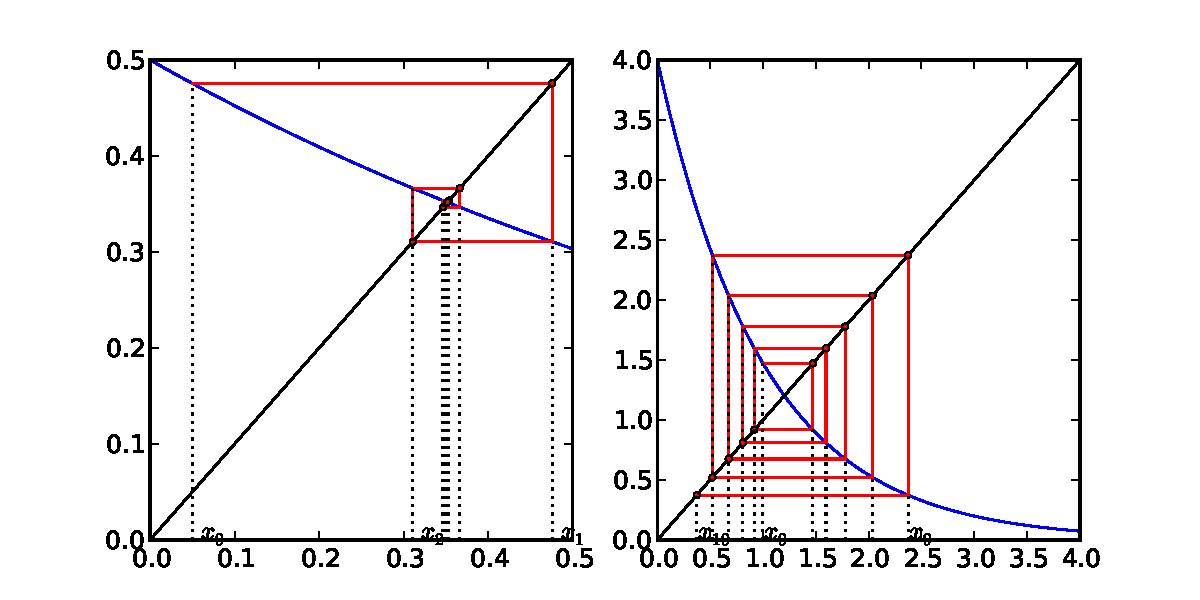
\includegraphics[width=\textwidth]{plots/banach}
  \caption{Sukzessive Substitution mit Funktion $g(r) = e^{-r}/\phi_0$
    mit $\phi_0=2$ (links) und $\phi_0=1/4$ (rechts). Blau
    durchgezogen ist die Funktion $g$, die Winkelhalbierende ist
    schwarz dargestellt. Die Punkte auf der Winkelhalbierenden
    markieren die Punkte $(x_1,x_1)$, $(x_2,x_2)$ usw., durch die das
    Lot auf $g$ gefällt wird, um den nächsten Punkt der sukzessiven
    Substitution zu erhalten. Im linken Graph sind die ersten sieben
    Glieder dargestellt, die exponentielle Konvergenz ist gut zu
    sehen. Im rechten Graph konvergiert das Verfahren nicht mehr.}
  \label{fig:banach}
\end{figure}

\subsection{Beispiel}

Als Beispiel für eine Anwendung des Banachschen Fixpunktsatzes
betrachten wir die dimensionslose Form des Yukawa- oder
Debye-Hückel-Potentials $\phi(r) = e^{-r}/r$. Wir fragen uns, wann für
welches $r$ dieses Potential einen gegeben Wert $\phi_0$ annimmt. Das
führt zu der Fixpunktgleichung
\begin{equation}
  g(r) = \frac{e^{-r}}{\phi_0} = r
\end{equation}
Die linke Seite ist eine auf $[0,\infty)$ L-stetige Funktion mit
$L=1/\phi_0$, wie man durch Ableiten leicht sieht.

Abbildung~\ref{fig:banach} zeigt die sukzessive Substitution für
$g(r)$. Graphisch lässt sich das Verfahren visualisieren, in dem in
jeder Iteration der Funktionswert $x_{n+1} = y =g(x_{n})$ an der
Winkelhalbierenden $y=x$ auf die $x$-Achse zurückgespiegelt wird. Im
linken Graph ist $\phi_0=2$ und damit $L=1/2$, so dass die sukzessive
Substitution exponentiell konvergiert. Für das letzte abgebildete
Glied, $x_7$, gilt $\abs{x_7-\overline{x}} \le 1/2^8 = 1/256$. Im
rechten Graph ist $\phi_0=1/4$ und damit $L=4$. Insbesondere ist auch
im Fixpunkt $g'(\overline(x))>1$. Abgebildet sind die ersten zehn
Glieder der sukzessiven Substitution, die hier nicht mehr
konvergiert. Wird hingegen $\phi_0$ so gewählt, dass 
$g'(\overline(x))<1$, aber $L>1$, so konvergiert das Verfahren zwar
noch, aber nicht mehr exponentiell.

\begin{figure}
  \centering
  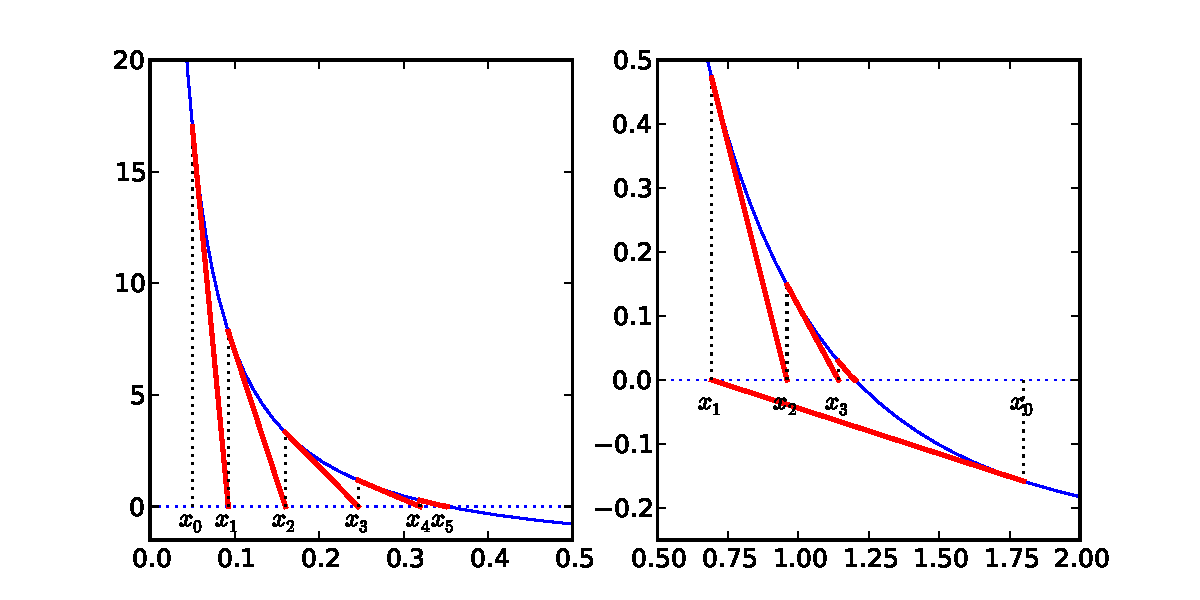
\includegraphics[width=\textwidth]{plots/newton}
  \caption{Newtonverfahren für die Funktion $f(r) = e^{-r}/r -
    \phi_0$. Wie schon beim Graphen zur sukzessiven Substitution ist
    links $\phi_0=2$, rechts $\phi_0=1/4$, allerdings konvergiert das
    Newtonverfahren für beide Werte. Blau dargestellt ist $f$, die
    roten, dicken Linien stellen die Tangenten dar, deren Nullstellen
    die neuen Näherungen für die gesuchte Nullstelle von $f$ sind.}
  \label{fig:newton}
\end{figure}

\section{Newtonverfahren in einer Dimension}
\index{Newtonverfahren}
\index{Nullstellensuche}

Nachdem wir bis jetzt die suzessive Substitution zur Bestimmung von
Fixpunkten betrachten haben, geht es nun um die Nullstellensuche. Sei
also zunächst eine stetig differenzierbare Funktion $f:[a,b]\to\RR$
gegeben und deren Nullstellen $x$, $f(x) = 0$, gesucht. Ähnlich wie
bei der sukzessiven Iteration starten wir mit einem Startwert
$x_0$. Um uns nun der Nullstelle der Funktion zu nähern, linearisieren
wir in der aktuellen Näherung $x_n$ und lösen nach der Nullstelle
$x_{n+1}$ auf:
\begin{equation}
  x_{n+1} = g(x_n) := x_n - \frac{f(x_n)}{f'(x_n)}\quad\text{für}\; n\ge 0,
\end{equation}
wobei wir annehmen, dass $f'(x)\neq 0$ auf $[a,b]$.  Für eine
Nullstelle $\overline{x}$ von $f$ gilt offenbar $g(\overline{x}) =
\overline{x}$, d.h. wir suchen einen Fixpunkt von $g$, den wir wieder
durch sukzessive Substitution annähern können. Man bricht das
Verfahren wie auch die sukzessive Substitution ab, wenn
$\abs{x_{n}-x_{n-1}}$ bzw. $\abs{f(x_n)}$ hinreichend klein sind.

Ist nun $f$ sogar zweifach stetig differenzierbar, so gilt
\begin{equation}
  g'(x) = 1 - \frac{f'(x)^2 - f(x)f''(x)}{f'(x)^2} =
  \frac{f(x)f''(x)}{f'(x)^2} \implies g'(\overline{x}) = 0.
\end{equation}
Das Newtonverfahren konvergiert also zumindest lokal gegen einen
Fixpunkt $\overline{x}$ von $g$ beziehungsweise eine Nullstelle von
$f$. Tatsächlich konvergiert das Verfahren wenigstens quadratisch,
wenn $f$ zweifach differenzierbar ist, da
\begin{align}
  x_{n+1} - \overline{x} = \frac{(x_n - \overline{x})f'(x_n) -
    f(x_n)}{f'(x_n)}
  = \frac{(x_n - \overline{x})}{f'(x_n)}\left( f'(x_n) -
    \frac{f(x_n) - f(\overline{x})}{x_n - \overline{x}}\right)\nonumber\\
  = \frac{(x_n - \overline{x})}{f'(x_n)}\left( f'(x_n) -
    f'(\xi')\right)
  = \frac{(x_n - \overline{x})^2}{f'(x_n)}f''(\xi)
\end{align}
und somit
\begin{equation}
  \frac{\abs{x_{n+1} - \overline{x}}}{\abs{x_n - \overline{x}}^2}
  \le \frac{\max_{\xi\in [a,b]} \abs{f''(\xi)}}{\max_{\xi\in [a,b]} \abs{f'(\xi)}}
\end{equation}
Ist $f$ nur differenzierbar, so lässt sich ähnlich zeigen, dass das
Newtonverfahren superlinear konvergiert. Das Newtonverfahren
konvergiert also in jedem Fall schneller als die sukzessive
Substitution, erfordert allerdings eine mindestens stetig
differenzierbare Funktion.

Bis jetzt haben wir nur die lokale Konvergenz des
Newton-Verfahrens. Ist die Zielfunktion $f\in C^1([a,b])$ allerdings
konvex bzw. konkav, also $f'$ monoton wachsend bzw. fallend, und hat
eine Nullstelle, so kann man zeigen, dass das Newtonverfahren global
gegen eine Nullstelle $\overline{x}$ von $f$ konvergiert. Dabei ist
das Verfahren nach dem ersten Schritt monoton, d.h. entweder $x_1\le
x_2\le\ldots\le\overline{x}$ oder $x_1\ge
x_2\ge\ldots\ge\overline{x}$.

\subsection{Beispiel}

Wir betrachten wieder die Aufgabe $e^{-r}/r = \phi_0$, bzw. $f(r) =
e^{-r}/r - \phi_0 = 0$. Die Ableitung dieser Funktion ist $-e^{-r}(1 +
r)/r^2$, $f$ fällt also monoton. Daher konvergiert das Newtonverfahren
global und monoton, wie in Abbildung~\ref{fig:newton} zu sehen. Im
linken Graphen ist $r_0<\overline{r}$, daher startet das Verfahren
sofort monoton. Im rechten Graphen ist $r_0 < \overline{r}$. Hier wird
im ersten Schritt $r_1 < \overline{r}$, und erst dann wächst die
Näherung wieder monoton. In jedem Fall konvergiert das
Newtonverfahren, anders als die sukzessive Substitution, für beide
Werte von $\phi_0$ innerhalb weniger Schritte zuverlässig gegen die
Nullstelle.

\subsection{Wurzelziehen}

Wir betrachten die Gleichung $f(x) = x^k - a = 0$ auf der positiven
Halbachse. Dann konvergiert für jeden Startwert $x_0>0$ das
Newtonverfahren
\begin{equation}
  x_{n+1} = x_n - \frac{f(x_n)}{f'(x_n)} = \left(1 -
    \frac{1}{k}\right) x_n + \frac{1}{k} \frac{a}{x_n^{k-1}}
\end{equation}
gegen die einzige Nullstelle, nämlich die $k$-te Wurzel aus
$a$. Sinnvollerweise wählt man daher $x_0=a$ als Startwert. Für $k=2$
ergibt sich das \emph{Heron-Verfahren} $x_{n+1} = \frac{1}{2}\left(x_n
  + \frac{a}{x_n}\right)$, das bereits im 2. Jhdt. vor Christus zum
Wurzelziehen benutzt wurde.

Für die Wurzel aus $a=2$ sind die ersten 5 Schritte des Heronverfahrens:
\begin{center}
  \begin{tabular}{r|l|l}
    Schritt $n$ & $x_n$ & Anzahl korrekter Stellen \\\hline
    0 & 1.000000000000000 & 1 \\
    1 & 1.500000000000000 & 1 \\
    2 & 1.416666666666667 & 2 \\
    3 & 1.414215686274510 & 5 \\
    4 & 1.414213562374690 & 11 \\ 
    5 & 1.414213562373095 & 15
  \end{tabular}
\end{center}
Mit der auf Rechnern üblichen doppelten Genauigkeit ist das Verfahren
damit konvergiert.

Die Anzahl der Rechenoperationen für $n$ Schritte entspricht der
Auswertung eines Polynoms mit $3n/2$ Koeffizienten. Wäre man zum
Beispiel nur an der Wurzel im Bereich $[0,5]$ interessiert und würde
hierzu eine interpolierendes Polynom mit 7 Chebyshev-Stützstellen
nutzen, wäre $\sqrt{2}\approx 1.40966$ mit gerade einmal einerq
korrekten Stelle. Mit einer Taylorentwicklung um 1 würde es etwas
besser. Bei 7 Termen liefert diese $\sqrt{2}\approx 1.4214$ mit 2
korrekten Stellen.

Für $k=-1$ wird aus der Wurzelaufgabe eine Division, da wir die
Nullstelle der Funktion $f(x) = \frac{1}{x} - a$ suchen. Die Lösung
kann nur mit Hilfe der Grundrechenarten durch die Iteration
\begin{equation}
  x_{n+1} = x_n - \frac{f(x_n)}{f'(x_n)} = 2x_n - a x_n^2 
\end{equation}
bestimmt werden. Allerdings ist die Ableitung von $a/x$ unbeschränkt,
daher konvergiert das Verfahren nur für Startwerte, die hinreichend
nah an der Lösung sind. Wie man sich in diesem Fall leicht überlegt,
konvergiert das Verfahren nur für $x_o\in (0, 2/a)$, was schwierig zu
erfüllen ist, ohne $a^{-1}$ bereits zu kennen.

\subsection{Nullstellen von Polynomen}

Ist $p$ ein Polynom, so lassen sich dessen Nullstellen (approximativ)
mit Hilfe des Newtonverfahrens bestimmen:
\begin{equation}
  x_{n+1} = x_n - \frac{p(x_n)}{p'(x_n)},
\end{equation}
wobei $p(x_n)$ und $p'(x_n)$ durch ein modifiziertes Hornerschema
bestimmt werden können:
\begin{lstlisting}[language=C]
double newton_step(double *series, int n, double xn)
{
  double p = c[n];
  double dp = n*c[n];
  for(int i = n-1; i >= 0; --i) {
    p  =  p*xn +   c[i];
    dp = dp*xn + i*c[i];
  }
  return xn - p/dp;
}
\end{lstlisting}
Das Newtonverfahren liefert natürlich nur eine Nullstelle des
Polynoms. Durch die Polynomdivision, wieder mit Hilfe des
Hornerschemas wie in Abschnitt~\ref{sec:horner}, lässt sich diese
aber abspalten und das Newtonverfahren erneut starten, bis alle
Nullstellen gefunden sind.

\section{Regula falsi}
\keyword{Regula falsi}

\begin{figure}
  \centering
  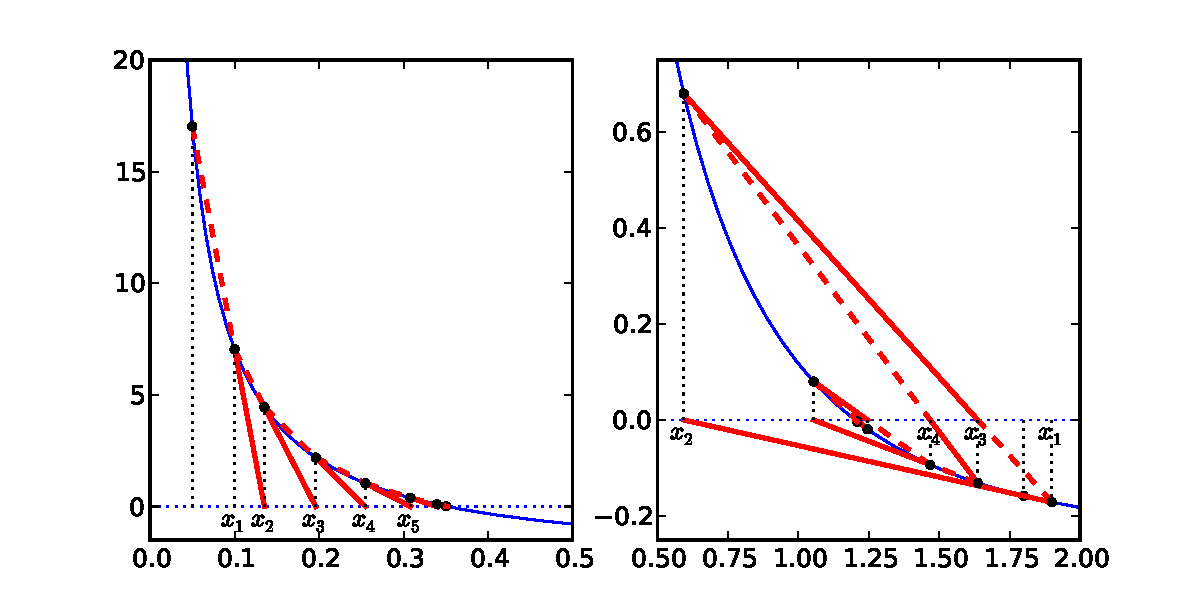
\includegraphics[width=\textwidth]{plots/regulafalsi}
  \caption{Regula falsi für die Funktion $f(r) = e^{-r}/r -
    \phi_0$. Wie zuvor ist links $\phi_0=2$, rechts $\phi_0=1/4$.
    Blau dargestellt ist wieder $f$, die roten, gestrichelten dicken
    Linien stellen die Sekanten dar, deren Nullstellen die neuen
    Näherungen für die gesuchte Nullstelle von $f$ sind. Durchgezogen
    ist der Abschnitt der Sekante durch $x_{n-1}$ und $x_n$, der von $x_n$
    zu $x_{n+1}$ führt.}
  \label{fig:regulafalsi}
\end{figure}

In vielen Fällen ist es nicht einfach oder unmöglich, die Ableitung
einer Funktion zu bestimmen. In diesem Fall kann man die Ableitung
durch die dividierte Differenz annähern, wobei nun zwei Startpunkte
$x_0$ und $x_1$ gebraucht werden. Daraus ergibt sich die \emph{Regula
  falsi}
\begin{equation}
  x_{n+1} = x_n - f(x_n)\frac{f(x_n) - f(x_{n-1})}{x_n - x_{n-1}},
\end{equation}
die nicht mehr quadratisch, aber wenigstens superlinear konvergiert.

Das Bestimmen der Ableitung von $f$ ist immer dann unmöglich, wenn $f$
sehr komplex ist. Ein Extremfall wäre eine
Molekulardynamik-Computersimulation, bei der zum Beispiel in
Abhängigkeit vom aktuellen Volumen $V$ der mittleren Druck $P(V)$ in
einem gegebenen System bestimmt wird. Den mittleren Druch nach $V$
abzuleiten, ist vollkommen aussichtslos, wenn die Wechselwirkungen
zwischen den Teilchen hinreichend komplex sind. Dabei ist es sehr wohl
von großem Interesse, dasjenige Volumen zu bestimmen, für das $P(V)$
gleich einem vorgegebenen Außendruck $P_0$ ist, denn dies ist die
natürliche Bedingung im isobarischen Ensemble. In diesem Fall ist
zusätzlich noch die Funktion $P(V)$ mit einer oftmals nicht kleinen
statistischen Unsicherheit belegt, weil die Druckschwankungen, also
die Varianz des Drucks, sehr groß sind. Trotzdem konvergiert die
Regula falsi im allgemeinen zufriedenstellend, solange keine zu hohen
Ansprüche an die Genauigkeit gestellt werden. Schliesslich kann die
Nullstelle nicht genauer als die vorhandenen Daten bestimmt werden.

Als Beispiel für die Regula falsi soll ein weiteres Mal die Funktion
$f(r) = e^{-r}/r - \phi_0$ dienen. Für diese zeigt
Abbildung~\ref{fig:regulafalsi} die erste paar Schritte der Regula
falsi. Unter geeigneten Umständen, nämlich, wenn die angenäherte
Tangente hinreichend gut mit der tatsächlichen über einstimmt,
konvergiert die Regula falsi praktisch genauso gut wie das normale
Newtonverfahren. Sind die Startpunkte allerdings ungünstig gewählt,
wie im rechten Beispiel, so kann es passieren, dass diese abwechselnd
um die Nullstelle liegen, und damit nicht mehr monoton konvergieren.

\section{Bisektion}
\index{Bisektion}
\index{Bisektionsverfahren}

Wie wir gesehen haben, konvergiert das Newtonverfahren und seine
Varianten sehr schnell, allerdings oft nur unter der Voraussetzung,
dass der Startwert hinreichend nah an einer Nullstelle liegt. Wie aber
kann man einen solchen Startwert finden? Hierfür wird ein langsameres,
robusteres Verfahren gebraucht, zum Beispiel das
\emph{Bisektionsverfahren} in einer Dimension.

Sei also wieder $f\in C([a,b])$ eine stetige Funktion, und
$f(a)f(b)<0$. Dann hat $f$ gemäß Mittelwertsatz wenigstens eine
Nullstelle im Interval $[a,b]$, die wir suchen. Dazu setzen wir
zunächst $a_0=a$ und $b_0=b$. Dann betrachten wir den
Intervallmittelpunkt
\begin{equation}
  m_{n} = \frac{a_n + b_n}{2}.
\end{equation}
Ist $f(m_n)f(a_n) < 0$, haben also unterschiedliche Vorzeichen, so
muss eine Nullstelle im halb so großen Interval $a_1=a_0$, $b_1=m_0$
liegen, mit dem wir nun weiter verfahren. Anderfalls ist
notwendigerweise $f(m_n)f(b_n)\le 0$, und die Nullstelle ist im neuen
Interval $a_1=m_0$, $b_1 = b_0$. Ist $b_n - a_n$ kleiner als die
gewünschte Genauigkeit für die Nullstelle, bricht man einfach
ab. $m_n$ ist dann die endgültige Näherung für die Nullstelle.

Das Verfahren halbiert in jedem Schritt die Intervallgröße und damit
auch den maximalen Abstand der Näherung zur tatsächlichen
Nullstelle $\overline{x}$. Es gilt als
\begin{equation}
  \frac{\abs{m_{n+1} - \overline{x}}}{\abs{m_{n} - \overline{x}}}\le \frac{1}{2},
\end{equation}
das Verfahren konvergiert also nur linear, dafür aber global.

In der Praxis kombiniert man die Bisektion mit dem Newtonverfahren, in
dem zunächst einige Schritte des Bisektionsverfahrens gestartet
werden, und dann vom Intervallmittelpunkt aus das
Newtonverfahren. Konvergiert dieses, so ist man fertig. Läuft das
Newtonverfahren hingegen aus dem Bisektionsinterval heraus,
verkleinert man dieses weiter durch Bisektion, und versucht dann
erneut, die Nullstelle mit dem Newtonverfahren zu bestimmen.

In Abbildung~\ref{fig:bisektion} dient uns ein letztes Mal die
Funktion $f(x) = e^{-r}/r - 2$ als Beispiel für die Bisektion. Mit
sieben Schritten schließt diese bei Startinterval $[0,1,\,1]$ die
Nullstelle bis auf $[0,3391,\,0,3461]$, als etwa $10^{-2}$ genau
ein. Zum Vergleich: das Newtonverfahren mit Startwert $0,05$ erreicht
in sieben Schritten eine Genauigkeit von etwa $10^{-5}$, und selbst
die Regula falsi $10^{-3}$.

\begin{figure}
  \centering
  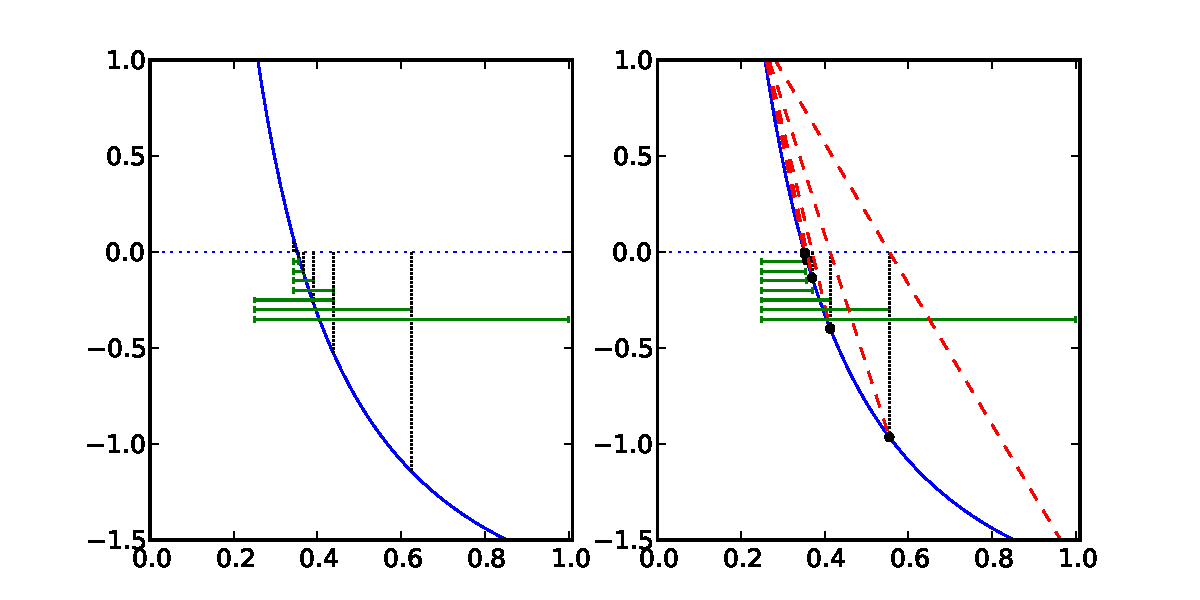
\includegraphics[width=0.5\textwidth]{plots/bisektion}
  \caption{Bisektion für die Funktion $f(r) = e^{-r}/r -
    \phi_0$, hier nur mit $\phi_0=2$, da die genau Form der Funktion
    für diese Methode unerheblich ist. Blau dargestellt ist wieder
    $f$, die roten Balken markieren die nacheinander generierten,
    kleiner werdenden Intervalle $[a_n, b_n]$, die der Sichtbarkeit
    wegen auf Höhe von
    $f(m_n)$ eingezeichnet sind. Die gestrichelten, schwarzen Linien
    markieren noch einmal ausdrücklichen die Intervalmitten $m_n$, die
    im nächsten Schritt eine der beiden Intervalgrenzen werden.}
  \label{fig:bisektion}
\end{figure}

\section{Newtonverfahren in mehreren Dimensionen}
\index{Gleichungssysteme>nichtlineare}

Bis jetzt haben wir das Newtonverfahren nur für eindimensionale
Funktionen betrachtet. Im mehrdimensionalen funktioniert das Verfahren
aber sehr ähnlich, wobei die Ableitung zur Jacobimatrix wird.

Sei also $f\in C^1(M, \RR^n)$ eine stetig differenzierbare Abbildung
von $M\in\RR^n$ in den $\RR^n$. Wir suchen nun eine Nullstelle
$\overline{x}\in D$, d.h. eine Lösung des nichtlinearen
Gleichungssystems $f(x) = 0$.

Wie schon im Eindimensionalen starten wir mit einer Näherung
$x^{(0)}\in M$, und berechnen die nächste Näherung $x^{(1)}$ durch
Linearisieren von $f$ in $x^{(0)}$. Die Linearisierung ergibt sich aus
der Taylorentwicklung:
\begin{equation}
  \label{eq:linnewton}
  F(x^{(1)}) \,\dot{=}\, F(x^{(0)}) +
  F'(x^{(0)})\left(x^{(1)}-x^{(0)}\right),
\end{equation}
wobei
\begin{equation}
  F'(x) = \left(\frac{d}{dx_j}F_k(x)\right)_{k,j} = 
  \begin{pmatrix}
    \frac{d}{dx_1}F_1(x) & \ldots & \frac{d}{dx_n}F_1(x)\\
    \vdots               &        & \vdots \\
    \frac{d}{dx_1}F_n(x) & \ldots & \frac{d}{dx_n}F_n(x)
  \end{pmatrix}
\end{equation}
die \emph{\keyword{Jacobimatrix}} von $f$ an der Stelle $x$ bezeichnet.
Die neue Näherung $x^{(1)}$ suchen wir als Nullstelle der
Linearisierung \eqref{eq:linnewton}, also aus der Bedingung
$F(x^{(1)})\stackrel{!}{=} 0$. Da wir ja damit nur die
linearisierte Gleichung gelöst haben, linearisieren wir erneut im
neuen Punkt $x^{(1)}$, und so weiter. Ein Schritt des Newtonverfahrens
ist dann also
\begin{equation}
  x^{(m+1)} = x^{(m)} + d^{(m)}\quad\text{mit}\;
  F'(x^{(m)})\,d^{(m)} = -F(x^{(m)}).
\end{equation}
Die \emph{Newtonkorrektur} $d^{(m)}$ wird als aus der Lösung eines
linearen Gleichungssystems gewonnen, zum Beispiel mit Hilfe der
Gaußelimination. Allerdings ist $f'$ im allgemeinen vollbesetzt, daher
verwendetet man normalerweise schnellere, approximative Verfahren, die
wir später kennenlernen werden. Ist $F'(x^{(m)})$ in einem Schritt
singulär, so bricht das Verfahren ab. Ansonsten wird weiter iteriert,
bis $\norm{d^{(m)}}$ hinreichend klein ist.

Auch im mehrdimensionalen konvergiert dieses Verfahren lokal
mindestens quadratisch, sofern in einer abgeschlossenen Umgebung der
Nullstelle $\norm{F'(x)^{-1}}$ beschränkt ist und $f$ zweifach stetig
differenzierbar. Allerdings gibt es kein langsames Verfahren ähnlich
der Bisektion, dass man dem Vefahren vorausschicken könnte, um die
Nullstelle einzugrenzen. Die globale Suche nach Nullstellen in
mehreren Dimensionen ist also eine schwierige Aufgabe. Eine
Möglichkeit ist, zunächst mit Hilfe von Optimierungsverfahren ein
$x_0$ zu finden mit möglichst kleiner Norm $\norm{f(x_0)}$, und von
dort das (gedämpfte) Newtonverfahren zu starten. Die globale
Optimierung in vielen Dimensionen ist selber eine sehr schwierige
Aufgabe, allerdings existieren hierfür Ansätze wie genetische
Algorithmen oder Simulated Annealing, die wir später kennenlernen
werden.

\subsection{Gedämpftes Newtonverfahren}
\index{Newtonverfahren>gedämpftes}

Leider ist im Mehrdimensionalen die Umgebung um die Nullstelle, in der
das Verfahren konvergiert, oftmals deutlich kleiner. Das Verfahren
springt dann leicht über die Nullstelle hinweg, wie es im
eindimensionalen nur am Anfang des Verfahrens vorkommt
(z.B. Abbildung~\ref{fig:newton} rechts, im ersten Schritt). Um dies
zu verhindern, kann man die Schrittweite reduzieren, als den Schritt
$d^{(m)}$ verkürzen. Die Iteration lautet dann
\begin{equation}
  x^{(m+1)} = x^{(m)} + \lambda d^{(m)}\quad\text{mit}\;
  F'(x^{(m)})\,d^{(m)} = -F(x^{(m)}),
\end{equation}
wobei die Dämpfung $\lambda\in (0,1]$ so gewählt wird, dass
$\norm{F(x^{m+1})}\le\norm{F(x^{m})}$. Dazu wird zum Bespiel mit
$\lambda=1$ begonnen, und $\lambda$ solange verringert, bis die
Bedingung erreicht ist.

\begin{lstlisting}[style=floating,deletekeywords={lambda}, float=t,
caption={Gedämpftes Newtonverfahren in mehreren
Dimensionen. \lstinline!f(x)! muß
eine vektorwertige Funktion sein, \lstinline!fprime(x)! ihre
Ableitung, d.h. eine matrixwertige Funktion.}]
# Gedaempftes Newtonverfahren
#############################

def gedaempfter_newton(f, fprime, x0, epsilon):
   xn = x0
   konvergiert = False
   while not konvergiert:
      # Newton-Korrektur
      dn = solve(fprime(xn), f(xn))
      if norm(dn) < epsilon:
         konvergiert = True
      else:
         # Schrittweitendaempfung
         lambda = 1.0
         abstieg = False
         while not abstieg:
            # neue Naeherung
            xneu = xn + lambda*dn
            if norm(f(xneu)) < norm(f(xn)):
               abstieg = True
            else:
               lambda = lambda / 2.0
         xn = xneu
   return xn
\end{lstlisting}

%%% Local Variables: 
%%% mode: latex
%%% TeX-master: "padc"
%%% TeX-PDF-mode: t
%%% End: 
